\documentclass{report}
\usepackage[utf8]{inputenc}
\usepackage{fullpage}
\usepackage[T1]{fontenc} 
\usepackage{fancybox} % for shadow and Bitemize
\usepackage{alltt}
\usepackage{graphicx}
\usepackage[colorlinks,hyperindex,bookmarks,linkcolor=blue,citecolor=blue,urlcolor=blue]{hyperref}
\usepackage{amssymb}
\usepackage{amsmath}
%\usepackage{wrapfig}
\usepackage{epsf}
\usepackage{listings}
\usepackage{multicol}

\title{\Huge{\textbf{DRAFT}}\\
\Huge{LU Decomposition with static pivoting strategy}}
\author{Omar ZENATI}
\date{\today}
         
\begin{document}
\maketitle
\begin{abstract}
This document aim to present a study on performance obtained on different versions of LU decomposition with a static pivoting strategy (getrf\_sp). First, a presentation of the LU decomposition is given with the two versions tested. After, the main performance results are described.
\end{abstract}
\tableofcontents

%-----------------------------------------------------------
\chapter{Introduction}

In scientific computing, the system of linear equation $Ax = b$ is often meeted. To resolve it, you have to compute the inverse matrix $A^{-1}$ which is too tedious. The alternative solution is to compute an LU decomposition of $A$ to resolve the equation $LUx = b$ which less complex to compute, where $L$ is a triangular lower matrix with the identity diagonal and $U$ is triangular upper matrix. Moreover, the LU decomposition have the advantage that $L$ and $U$ may be stocked in place of the $A$ matrix (the Identity diagonal is not stocked).

\section{LU Decomposition Algorithm}
This chapter present two approach of LU decomposition : a blocked version and a recursive. Both use the same strategy of pivoting which is the static pivoting. In this section, I present first the naive algorithm of LU decomposition. Then, I explain the static pivoting strategy. Finally, I describe the two versions compared.

\subsection{The naive algorithm}
The LU decomposition is based on the Gauss method. The algorithm is:
\begin{verbatim}
GETF2(A)
=================================================================
For k from 1 to min(A.m,A.n)
   Search for a pivot then do pivoting
   For i from k+1 to A.m
      a(i,k) = a(i,k)/a(k,k)    /*scale operation*/
   For i from k+1 to A.m
         For j from k+1 to a.n
            a(i,j) = a(i,j)-a(i,k)*a(k,j)   /*ger operation*/
=================================================================
\end{verbatim} 
\subsection{The static pivoting strategy}
The pivoting consist to research the maximum on the current column and after to swap its line with the current line. This operation is made to preserve the order of the matrix elements. However, it consume a lot of performance because it create a sort of barrier. An alternative solution is to define a criteria, and at each \texttt{k} of the loop, if the criteria is higher than \texttt{A(k,k)} then it remplace it. With this solution, the matrix resulted is not the exact solution, but it may be used as an entry for iterative methods. In the rest of the document, the function which apply the naive algorithm with static pivoting will be called \texttt{GET2F\_SP}.
\subsection{The blocking version}
In the naive algorithm, the performance may be optimized. In fact, because the operations are BLAS 1 level (scale) or BLAS 2 level (ger), there is a huge latency due to cache access. So, the idea is to make operations on blocks in place of lines and columns. This will make possible to use BLAS 3 level operations which are more efficient.\\
\begin{figure}[!h]
\begin{center}
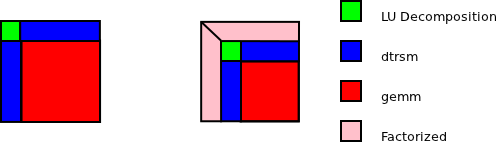
\includegraphics[width=\textwidth]{lu_decomposition_block.png} 
\end{center}
\caption{dgetrf\_sp performance results on AMD architecture}
\end{figure}

The algorithm of LU decomposition by block is :
\begin{verbatim}
GETRF_SP(A)
=================================================================
/* SB is the size of block defined */
For k from 1 to min(A.m/SB,A.n/SB)
   GETF2_SP(A(k,k))   /*LU Decomposition*/
   For i from k+1 to A.m/SB
      TRSM_U(A(k,k),A(m,k))
   For i from k+1 to A.m/SB
      TRSM_L(A(k,k),A(k,n))
   For i from k+1 to A.m/SN
      For j from k+1 to A.n/SB
            GEMM(A(i,k),A(k,j),A(i,j))
=================================================================
\end{verbatim}
\subsection{The recursive version}
As it is shown in the blocking version, there is a need for a defined size of block. The choice of the size may affect the performance. An alternative solution is to use a recursive algorithm which will divide into two part the matrix at each iteration. The numbers of BLAS 2 level of operation is divided into two. So,the recursive algorithm is :

\begin{verbatim}
GETRF_SP_REC(A)
=================================================================
/* SB is the size of block defined */
if(A.m >0)
   if(A.n == 1)
      Pivoting to criteria if necessary
      SCAL(A(0,0),A.column(0))
   else
      GETRF_SP_REC(A.leftHalf())
      TRSM_U(A.upLeftQuarter,A.uprightQuarter)
      GEMM(A.downLeftQuarter,A.uprightQuarter,A.downRightQuarter)
      GETRF_SP_REC(A.downRightQuarter())
=================================================================
\end{verbatim}


\section{Performance results}
The test of performance was made on an AMD Opteron(tm) Processor 6168
which turn at 1900.209 MHz. The benchmarks concern the two precisions : double and simple. The results obtained are described in the two figure below.
\begin{figure}[!h]
\begin{center}
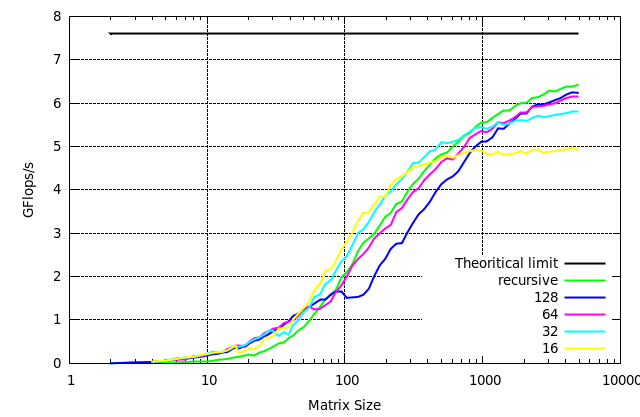
\includegraphics[width=\textwidth]{exp_dgetrf_sp_amd.png} 
\end{center}
\caption{dgetrf\_sp performance results on AMD architecture}
\end{figure}

\begin{figure}[!h]
\begin{center}
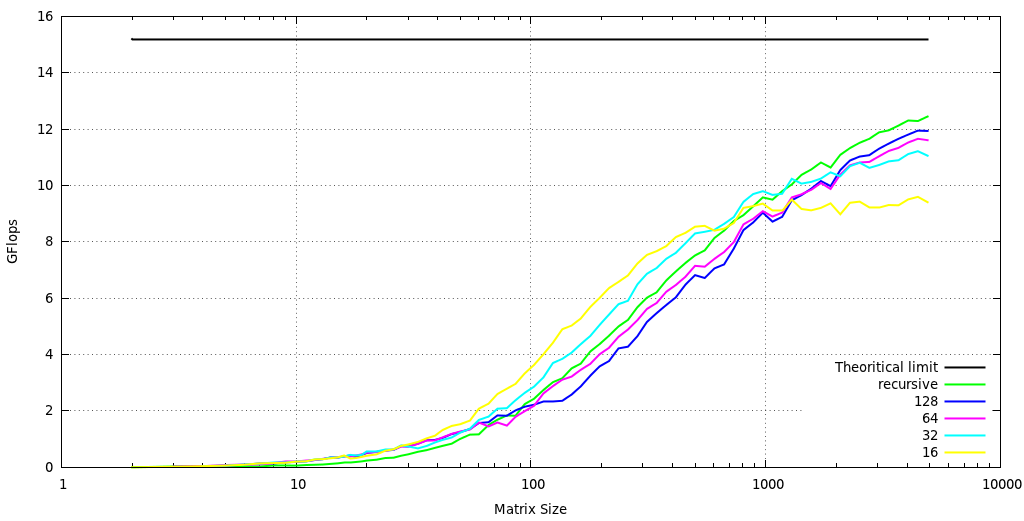
\includegraphics[width=\textwidth]{exp_sgetrf_sp_amd.png} 
\end{center}
\caption{sgetrf\_sp performance results on AMD architecture}
\end{figure}

\chapter{DAGuE}

Nowadays, the architectures of clusters are more and more heterogeneous and hybrid. Whether it be CPU or GPU, their number increase progressively.
\begin{figure}[!h]
\begin{center}
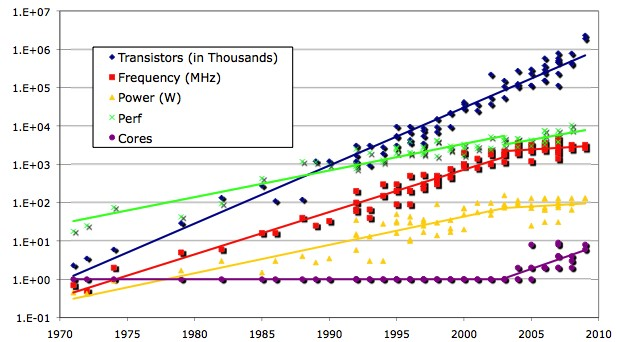
\includegraphics[width=\textwidth]{increase.png} 
\end{center}
\caption{Evolution of some curve last 40 years}
\end{figure}
Cluster gained in performance but their use gain in complexity. In order to ease their operating, computer science engineer design software that introduce an abstraction to these architectures. These softwares are called \textbf{\textit{Runtimes}}. Their rules is to detect the architecture used and schedule tasks on it in the best way. Today, some runtimes are famous :
\begin{itemize}
\item StarPU: developed by Runtime (Inria) in Bordeaux, FRANCE
\item StarSS: developed by BSC in Barcalona,SPAIN
\item DAGuE: developed by ICL in Tennessee, USA
\item Quark: developed by ICL in Tennessee, USA
\item Cilk: developed by MIT in Massachusetts, USA
\item TBB: developed by Intel.
\end{itemize}
In this study, I will focus on DAGuE. DAGuE is a Direct Acyclic Graph (DAG) scheduling engine, where the nodes of a DAG are sequential computation tasks and the edges are data communications. To design a parallel application with DAGuE, each task is implemented sequentially into a kernel with a DAGuE specific language. It is also required to specify the data dependence between each task.

\section{GETRF\_SP on DAGuE}
In this section, an implementation of getrf\_sp on DAGue is presented as example. To implement a DAG of tasks, the language used on DaGuE is the JDF format. The JDF is a collection of functions definition where each one include :
\begin{itemize}
\item definition space;
\item task distribution;
\item set of data dependencies;
\item body to be executed (written in language C).
\end{itemize}
The figure below show the jdf code of zgetrf\_sp (the fourth item is not showed).
\begin{figure}[!h]
{\scriptsize\lstinputlisting[multicols=2,numbers=left,language=C]{zgetrf_sp.jdf}} 
\caption{JDF representation of LU decomposition}
\end{figure}

\begin{figure}[!h]
\begin{minipage}[!h]{.5\linewidth}
\centering
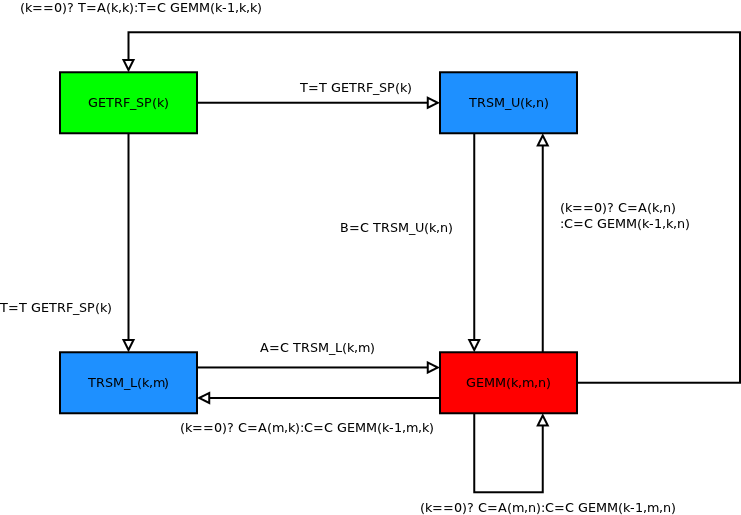
\includegraphics[width=\textwidth]{dag_getrf_sp.png}
\caption{Data interaction between kernels}
\end{minipage} \hfill
\begin{minipage}[!h]{.5\linewidth}
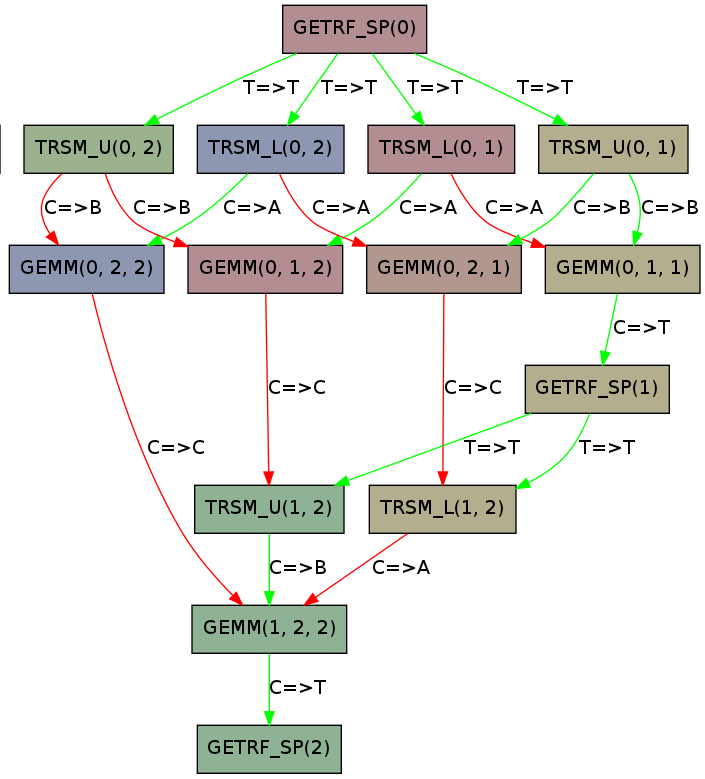
\includegraphics[width=\textwidth]{dag.png}
\caption{DAGuE dgetrf\_sp on a matrix with size of 500 and a tile of 200}
\end{minipage}
\end{figure}

\section{Performance results}

\begin{figure}[!h]
\begin{center}
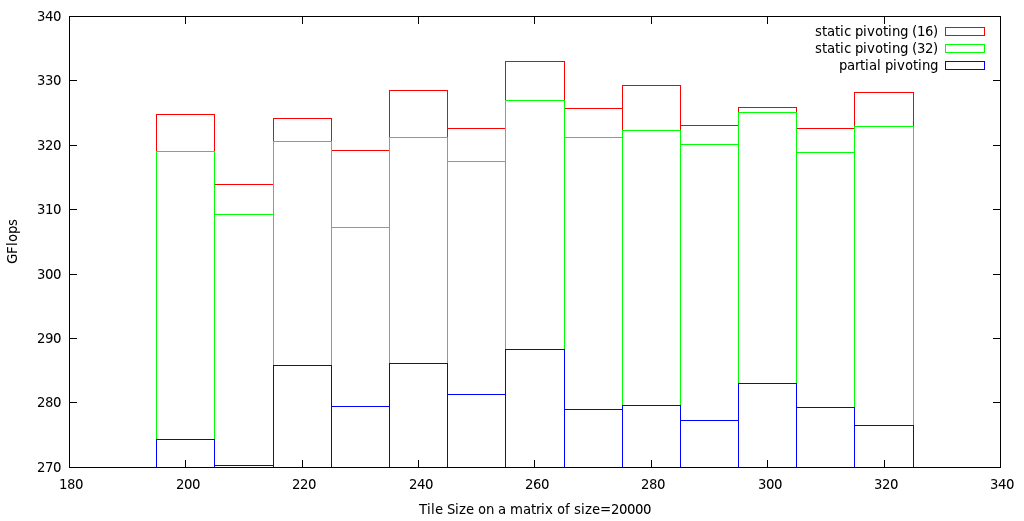
\includegraphics[width=\textwidth]{dgetrf_dague_remus_tile.png} 
\end{center}
\caption{LU decomposition on shared memory}
\end{figure}


\begin{figure}[!h]
\begin{center}
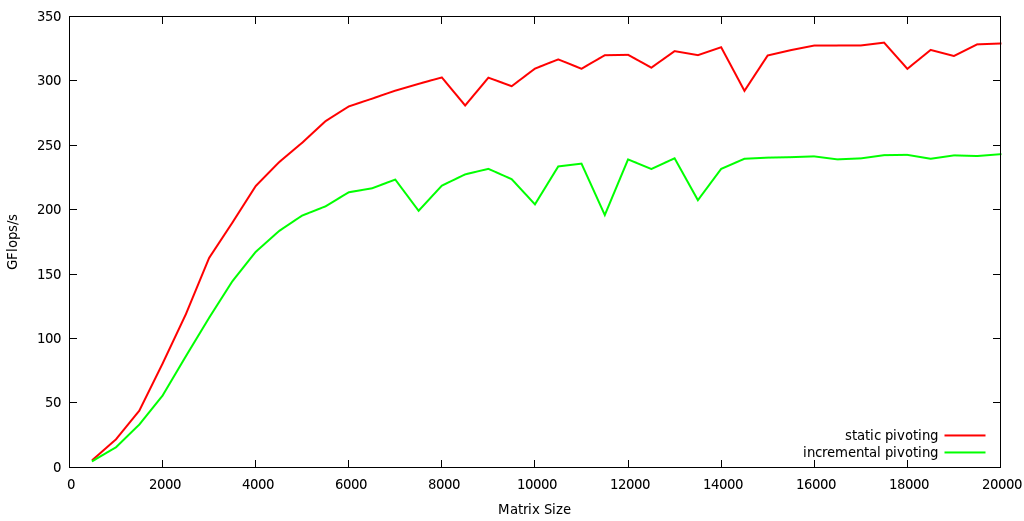
\includegraphics[width=\textwidth]{dgetrf_dague_remus.png} 
\end{center}
\caption{LU decomposition on shared memory}
\end{figure}

\chapter{Iterative refinement}
As said in the introduction, the Lu decomposition with static pivoting is most used to get an initial solution. Then, this is used iterative refinement. In this chapter, I explain the iterative method. But first, I present the way to define the criteria used in the GETRF\_SP.

\section{Definition of the criteria}
The criteria is the value used to compare the current pivot. If the criteria is higher than the current pivot, then it replace it. The user can initialize this criteria by any value. But, the most general value which can preserve the matrix order is the norm of the matrix multiplied by the epsilon of current precision.
\section{The iterative refinement}
The iterative refinement is a method to converge - after an series of loop - from a perturbed solution to a more accurate solution. So, from an initial inputs data $A$ and $B$, you try to resolve :
\begin{center}
$AX=B$
\end{center}
An first perturbed solution $\tilde{X}=X+\delta{X}$ is obtained. The idea is to multiply the matrix $A$ by the perturbed solution :
\begin{center}
$A\tilde{X}=A(X+\delta{X})=B+\delta{B}$
\end{center}
So, you obtain a new equation :
\begin{center}
$A\delta{X}=\delta{B}$
\end{center}
Resolving this equation provide a new perturbed solution $\widetilde{\delta{X}}$ of the lag $\delta{X}$. By subtracting it to $\tilde{X}$, you obtain a better perturbed solution $\tilde{\tilde{X}}$ to $X$.\\
More you reiterate this process, more you will obtain a better solution. The limit will be the epsilon of the used precision.\\
These mathematical formula can be summarized by the following algorithm :
\begin{enumerate}
\item Compute an initial solution $X_0$ from the linear system $AX=B$
\item Compute the residual $R_n=B-AX_n$
\item Resolve the linear system $AZ=R_n$
\item $X_{n+1}=X_n+Z$
\item If $\Vert{Z}\Vert/\Vert{X_{n+1}}\Vert<eps$ then STOP else goto 2
\end{enumerate}
The equivalent algorithm in the syntax used in this document is :
\begin{verbatim}
GETRS_SP(A,B)
=================================================================
COPY(A,LU)
GETRF_SP(LU)
COPY(B,S)
GETRS(LU,S)   /* (1) */
Do
   COPY(B,R)   
   GEMM(-A,S,R)   /* (2) */
   GETRS(LU,R)   /* (3) */
   AXPY(R,S)   /* (4) */
While(||R||/||S||>eps)   /* (5) */
B=S   /* Stock the result on B */
=================================================================
\end{verbatim}

\end{document}